\chapter{Google Architecture}
\label{chap:google_architecture}

Google is one of the well-known examples of corporations that deal with Big Data.
Its activity directly relates to storing and processing of large volumes of data.
Google Search engine handles more than three billion searches every day.
Social networking service Google+ had 540 million users in 2013.
Gmail, Google's email service, had 425 million users in 2012.
These are just several examples of large-scale Google projects, that processes huge amounts of data.
Therefore, Google introduces a batch of solutions for building scalable systems. 

The overall structure of Google Big Data architecture is presented on the
Figure~\ref{fig:google_architecture}.
The lowest layer is Linux kernel, that serves as a basis for Google File System.
Google File System is a scalable and highly available file system. 
These properties are achieved by replicating data across several machines.
Next, data can be efficiently processed by MapReduce framework.
This technology includes two steps - map, that performs filtering and sorting and reduce, that aggregates the output of map step to the final result.
Bigtable, a highly scalable database, provides a way to store massive amounts of information.
Finally, client application uses these technologies to perform highly scalable and distributed tasks.  
Let us explain in more detail the primary features and internal structure of these technologies.

\begin{figure}
  \centering
  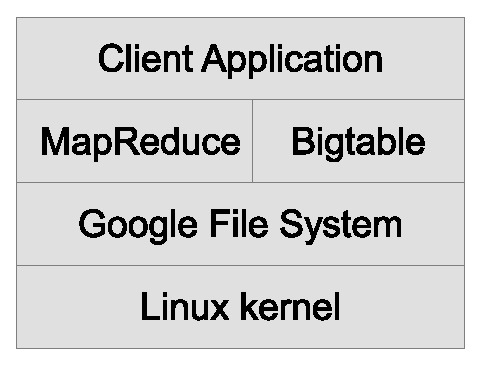
\includegraphics [width=0.4\textwidth]{images/Google_architecture}
  \caption{Google Architecture}
  \label{fig:google_architecture}
\end{figure}

\authorsection{Google File System}{SP}
[reference]
\mnote{Google File System}
Google File System (GFS) is a scalable distributed file system, which supports Big Data operations.
The underlying idea is the following: Google Search Engine and some other Google systems process vast amount of data, which is spread all over the world.
Hence the file system should be highly extensible, give an opportunity to use cheap hardware components and, consequently, be fault tolerate. 
Furthermore, it has some specific usage features.
Because of vast scales and cheap hardware, component failure is a commonplace.
The size of files exceeds several-fold the traditional standards, so a multi-gigabyte file is not unusual.
Most of the time the stored data stays unchanged and new data is only appended.
The append operation, in its turn, should provide the concurrent access for multiple clients.
GFS architecture design helps to meet all these requirements.

The Figure~\ref{fig:GFS_architecture} illustrates the main components of the GFS
Architecture.
Each GFS cluster contains one master server and several chunkservers.
The master has a "shadow" node, that provides read-only access when the primary master is down. 
Chunkserver stores chunks as Linux files on local disk.
Every chunk is replicated on several chunkservers for reliability.
One chunk combines multiple files and has a fixed size of 64 megabytes.

% Figure: according to [66]
\begin{figure}
  \centering
  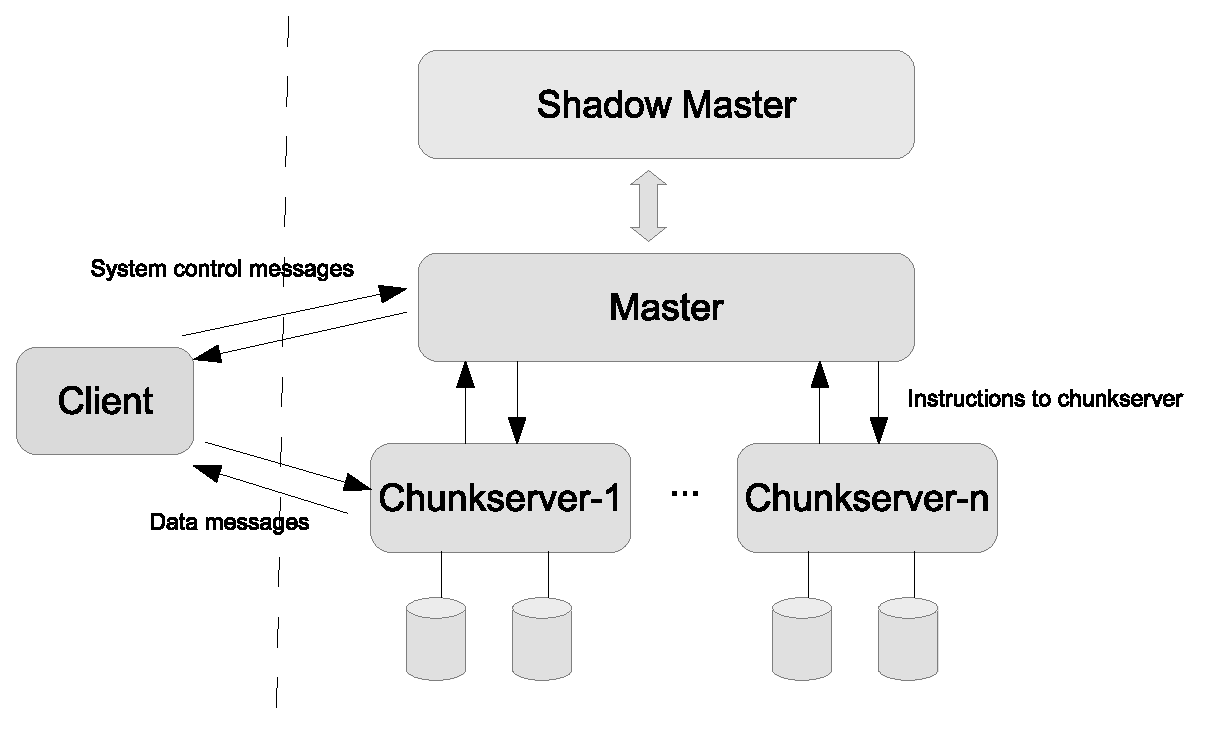
\includegraphics [width=0.8\textwidth]{images/GFS_architecture}
  \caption{GFS Architecture}
  \label{fig:GFS_architecture}
\end{figure}

The large size of chunk gives several advantages.
Clients send requests to the master for chunk location less frequently.
A persistent TCP connection to the chunkserver for a longer time period allows to avoid network overhead.
The master node stores less metadata that provide a possibility to keep it in memory.

The master node manages the mapping from files to chunks, location of chunks, access control, garbage collection and some other tasks.
It does not persistently store the information about chunks location. 
On the contrary, it gives instructions to chunkservers and collects their states using periodic HeartBeat messages.
To prevent the master being a bottleneck, only file system control data goes through it.
For example, a client can ask the master node which chunkservers it should contact.
The master node returns the corresponding chunk handle and its replicas' location.
After receiving a reply, the client caches this information and can directly transfer data to the given chunkserver, dispensing master node from overload.
Clients and chunkservers do not cache file data.
Clients mostly work with files that are too large to be cached.
Chunkservers treat chunks as Linux files, therefore in this case caching is done by operating system.

\mnote{Operation Log}
To recover its state, the master uses the operation log.
The operation log consists of the chronometric information about critical metadata changes.
This log is replicated on several machines.
For the purpose of consistency, client receives a respond for operation only when corresponding log record is flushed to a local disk and the disks of all replicas.
To avoid the operation log being too large, the master makes a checkpoint each time when the log size exceeds a certain threshold.
In the case of failure, the master can load the latest checkpoint from local disk and replay it, recovering its state.
For storing checkpoint it uses a compact B-tree like data structure, that allows to map it directly into memory and perform fast lookups.
For performance reasons the new checkpoint is created in separate thread.
The ability of a server to restore its state does not depend on the way it was terminated.
Shutting down a server by killing the process is a normal procedure. 

\mnote{Mutation}
A mutation denotes a change of the contents or metadata of a chunk.
There are two types of mutations, namely writes and record appends.
In the former case data is written with a file offset specified by a client.
In the latter, GFS chooses an offset, and data (record) is appended with an append-at-least-once semantics.
Record append operation is atomic, i.e. it is treated as one continuous sequence of bytes. 
This allows multiple clients to append information concurrently.

\mnote{Lease}
Each mutation is replicated across several chunks.
To keep a mutation order consistent at all the replicas, GFS uses a technique of leases.
The master gives a lease to one of the replicas, that becomes a primary replica.
The primary chooses an order for all the chunk's mutations and each replica then follows this order when applying mutations.

The flow of write control is shown on the Figure~\ref{fig:write_control_flow} in
more details.

\begin{figure}
  \centering
  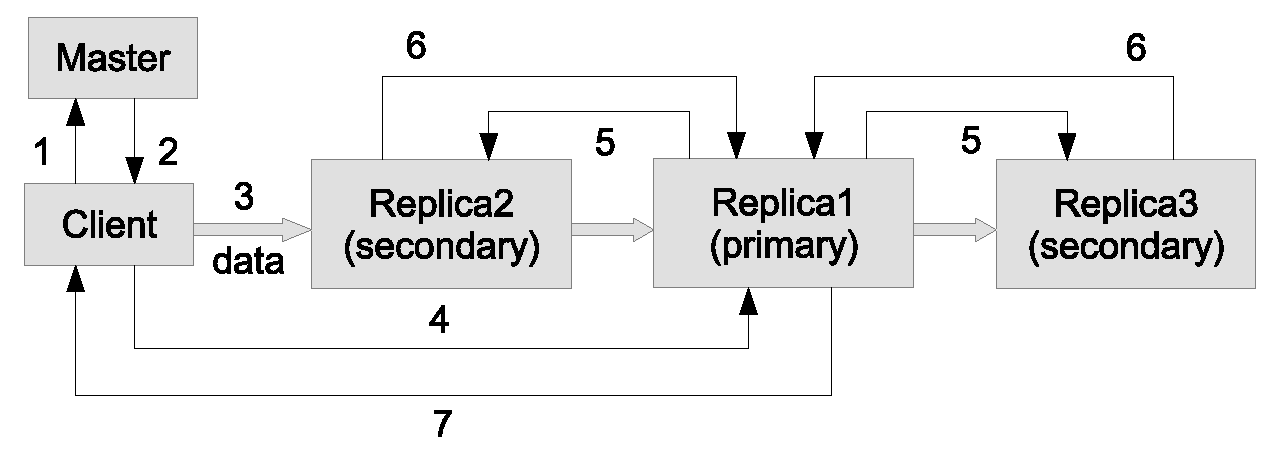
\includegraphics [width=0.7\textwidth]{images/write_control_flow}
  \caption{Write control flow}
  \label{fig:write_control_flow}
\end{figure}

1. The client sends a request to the master.

2. The master replies with a chunkserver, that holds the current lease, and the location of the other replicas.
If a primary replica (that has a lease) is not defined, the master chooses one. 
The client caches this information for the next mutations.

3. The client sends the data to all the replicas in arbitrary order.
Chunkservers store this data in an internal buffer cache. 

4. When the client receives acknowledgements from all the replicas, it sends a write request to the primary.
The primary picks serial numbers to all the mutations it has received and performs them in corresponding order.

5. All secondary replicas receive the write request forwarded by the primary.
Each replica applies mutations to its own state in the same order assigned by the primary.

6. The secondaries notify the primary about the completion of the operation.

7. The primary sends a reply to the client.
In the case of error occurrence at any of the replicas, the primary informs the client about them.
The write is considered to be successful, if the primary and an arbitrary number of secondary replicas succeeded.

GFS differs from traditional file systems in the way how it manages files and directories.
There is no possibility to list all the files in a directory in GFS, because it does not support per-directory structure.
It stores a mapping between full pathnames and metadata in a lookup table.
Prefix compression helps to efficiently represent this table in memory. 

The file deletion does not occur at once.
Firstly the master logs the event of deletion.
Than the system renames the file with a hidden name that includes the time of deletion.
The master performs a regular scan of the namespace and removes a hidden file, if it has existed for more than a specified time interval (e.g. 3 days). 

All the described features help the Google File System to successfully cope with a large-scale data processing workload.
GFS meets the storage needs of Google corporation.
Therefore Google uses GFS as the storage platform for many applications, both in research and production areas.
Another Google technologies, like MapReduce or BigTable are based on it.  	 

\authorsection{MapReduce}{SP}
\label{sec:mapreduce}
[reference]
MapReduce model finds wide application in a variety of real world tasks.
For example, search engines use web crawling to gather a vast amount of information.
They process this information to create inverted indices, construct web graphs, figure out the most frequent search queries, etc.
Any of these tasks can be divided into two steps, namely Map and Reduce.
Map operation converts input data to a set of intermediate key/value pairs.
Reduce operation, in its turn, combines all the values that share the same key.
The advantage of the MapReduce abstraction is that it hides the implementation details from users.
This allows even not experienced programmers to easily construct parallel and distributed systems.

MapReduce shares the same requirements with other systems that work with large data sets.
It should provide high parallelization, be fault-tolerant and perform load balancing between nodes.
Applying Map and Reduce operations helps to parallelize large calculations.
Moreover, this makes simpler re-execution of a task that serves as a primary mechanism for fault tolerance.

Both Map and Reduce operations work with key/value pairs.
The user of MapReduce library determines the logic of these operations, specific to the given application.
The Map function receives an input a key/value pair and produces a set of intermediate pairs.
The MapReduce library groups these intermediate pairs together by the key and passes the result to the Reduce function.
It passes them via iterator that allows to handle a large data set without keeping it in memory.
The Reduce function merges the values with the same key, possibly decreasing a given set of values.
One Reduce function invocation most of the time produces a single output value, or even none.
A pseudo-code for a simple MapReduce task is illustrated in Listing~\ref{lis:simple_mapreduce_task}.

\begin{lstlisting}[caption=Simple MapReduce task, label=lis:simple_mapreduce_task]
def map(key, value):
	list = []
	for x in value:
		if some_condition_holds:
	 		list.append((key, x))
	return list

def reduce(key, list_of_values):
	result = 0
	for x in list_of_values:
		result += x
	return (key, result)
\end{lstlisting}

\begin{figure}
  \centering
  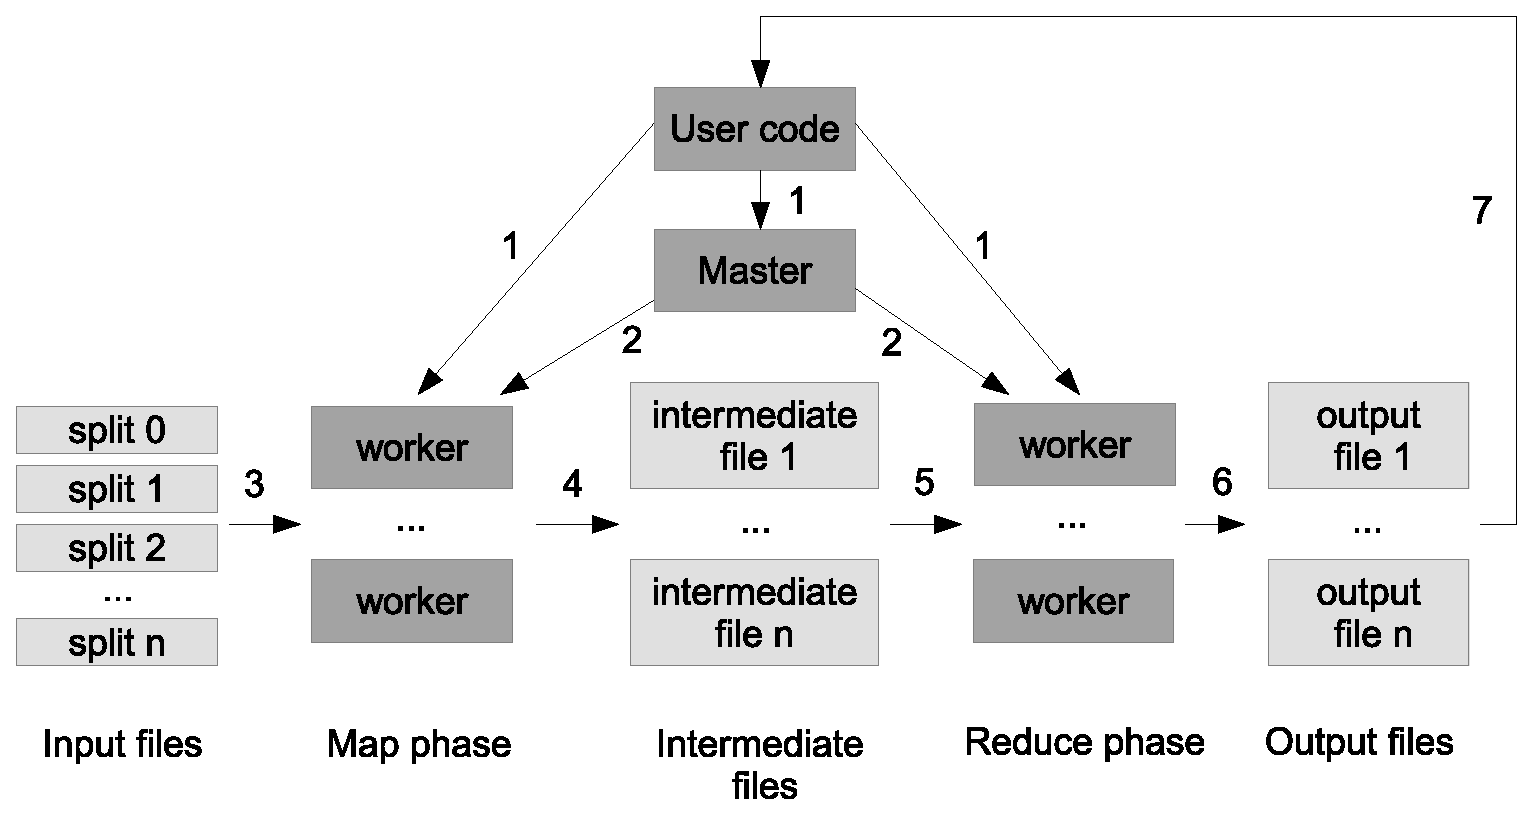
\includegraphics [width=0.9\textwidth]{images/MapReduce_operation_flow}
  \caption{MapReduce operation flow}
  \label{fig:mapreduce_operation_flow}
\end{figure}

We visualize the overall flow of a MapReduce operation in the Figure~\ref{fig:mapreduce_operation_flow}.

1. The MapReduce library divides the input files into M splits.
The size of one piece varies from 16Mb to 64Mb depending on the chosen settings.
User code invokes the MapReduce routine on several machines.

2. One of these machines is a master, while others are workers.
The master manages the workers, assigning to idle nodes one of M map tasks or one of R reduce tasks.

3. A worker that handles a map task reads the data from a respective input split.
It passes the parsed key/value pairs to the Map function.
The intermediate output of the Map function is stored in a buffer.

4. The MapReduce library periodically writes the buffered data into selected number of R local intermediate files.
Also it informs the master about the location of these files.

5. The master passes the locations to workers that handle a reduce operation.
A reduce worker reads the intermediate pairs from a specified location using remote procedure calls.
After compliting the reading, the worker groupes together all the pairs that share the same key.

6. These pairs are then passed to the Reduce function, one key and one or several related values at a time.
The output of the Reduce function is written to one of the output files.

7. After finishing all the map and reduce tasks, the MapReduce library returns the control to the user code.
The derived output files can be directly processed or be used as an input to another MapReduce task.

The MapReduce library has an optional Combine function that can be used for optimisation.
For example, let us consider the task of counting the number of words in English text.
Most probably it contains a lot of articles `a` and `the`.
Each Map task sends thousands of pairs <a, 1> to a single Reduce operation over the network. 
The Combine function can improve this situation by partial merging these pairs before sending them over the network.
Each machine that executes a Map function now also executes a Combine function.
Combine operation often uses the same code as Reduce one.
The difference is that the output of the former is stored in an intermediate file, while the latter writes it into the final output file.

The usage of Google File System (GFS) for storing input data helps to reduce the network bandwidth consumption.
GFS stores input data in blocks, copying each block on different machines (usually it makes 3 copies).
The master in MapReduce library knows which machine contains a replica and tries to assign a corresponding map task to this machine.   
When it is not possible, the master uses the nearest node to that machine.
This technology conserves network bandwidth significantly, especially when dealing with huge MapReduce operations.
 
The master keeps track of worker failures.
For this purpose it stores the state of each task and the identity of the worker that performs the task.
There are three types of states: idle, in-process and completed.
The behavior of the master in the case of failure depends on the type of the task (map or reduce) that failed.
When the map task fails, the master re-executes it on another worker.
Re-execution is required since the output of the map task is stored locally on the failed machine.
On the contrary, there is no need to re-execute the reduce task because global file system stores its output.
Sometimes a failure is caused by a defective record.
In this case the MapReduce library optionally can skip this record to continue the work. 
 
Stragglers is another problem that can obstruct the task completion.
Straggler is a machine that handles the last several map or reduce tasks too slow, keeping the whole system waiting for completion.
The MapReduce master uses a special mechanism to solve this problem.
On termination of an operation it executes the remaining in-process tasks on two different machines.
When either primary or backup worker completes computations, the task is considered to be completed.

Google Search engine widely uses MapReduce functionality for indexing, computing different statistics and analysing data.  
Moreover MapReduce can significantly facilitate the problems of data mining and machine learning.
Its key feature of dividing the computation into Map and Reduce phases helps to easily build distributed systems and makes the computation considerably more efficient.  

\authorsection{BigTable}{SP}
[reference]
Some Google projects deal with so large amounts of data, that common storage systems cannot sustain such a load.
For instance, personalized search, that stores user browser history and handles search queries based on the stored information about user activity.
It is necessary to warehouse each user's data.
Taking into account the huge number of Google Search users, the amount of data to be stored is also tremendous. 

The company introduces its own storage system for these purposes - a Bigtable.
It is a sparse, distributed, persistent multidimensional sorted map. [reference]
Bigtable uses three-dimensional mapping: row key, column key and timestamp are mapped to an array of bytes.
It is created to store petabytes of data in a distributed way.
As Google uses Bigtable in various projects, it puts different requirements on data size and latency of the storage system. 

\mnote{row keys}
The row key is represented by an arbitrary string with a maximum size of 64Kb.
Read and write operations under one row key are atomic.
Bigtable stores row keys in lexicographic order and dynamically partitions each row range.
One partition is called a tablet and serves as a distribution and load balancing unit.
For instance, when storing web pages with an URL as a row key, it is optimal to arrange pages from the same domain in one tablet.
In this case an URL like en.wikipedia.org/index.html is presented as org.wikipedia.en/index.html.

\mnote{column keys}
Bigtable groups column keys into column families, which serves as an access control units.
It means that each column family can have different access permissions (e.g. write access for one application and read only for another one).
It is common to store in one column family data of the same type.
One can store data under a column key only when a column family comprising this column key is created.
Number of distinct column families should be kept small, while each column family can contain unbounded number of columns.
The name of column key is presented as family:qualifier pair, where family should be printable and qualifier can be an arbitrary string.
For example, the column key name can look like language:en, where 'language' is a column family name and 'en' is a language ID. 

\mnote{timestamps}
Timestamps are used to store multiple versions of the same information.
A timestamp can be assigned in different ways.
On the one hand, Bigtable can use the time in microseconds as a timestamp.  
On the other hand, a client application can maintain its own unique timestamps.
Several versions of data are ordered such as the most recent version can be accessed first. 
Garbage collector processes the outdated data automatically using one of the two column family settings to detect the outdated versions.
The first setting allows to keep only the last \textit{n} versions of data, while the second setting allows to keep data that was written in the last \textit{m} days.

\mnote{Sawzall}
Bigtable allows user to manipulate the stored data using a special language developed by Google.
The language is called Sawzall.
Scripts, written in this language, can execute on Bigtable server's address spaces.
Using Sawzall scripts one can filter, transform and make various summarization on data.

\mnote{Chubby}
Chubby is a persistent distributed lock service for synchronizing access to shared system resources.
The Chubby service replicates to five nodes, choosing one of them to be a master node.
The service provides a namespace, that contains directories and files, and uses them as a lock.
Chubby has a client library that can keep the cached Chubby files in memory.
Every client sustains a session with Chubby service.
The expired session loses all the locks.

Bigtable uses Chubby for several purposes.
First, Chubby guarantees to have at most one active master at a time.
Second, it handles the appearance of new tablets and finilizes the dead ones.
Third, it stores the schema of Bigtable and access control lists.

The major components of Bigtable are a master server, a number of tablet servers and a library linked into each client.
It is possible to dynamically add or remove tablet servers according to given workload.
The master assignes tablets to tablet servers, performs load-balancing, garbage collection.
Furthermore, it is responsible for creation of tables and column families.
Each tablet server controls a tablets set.
When a client sends a read or write request to the tablet, this request is processed by the tablet server.
Also the tablet server splits too large tablets.

The internal details of master-slaves interaction are similar to those mentioned above in GFS and MapReduce subchapters.
Analogously, the system does not transfer client data through the master and establishes a direct connection between clients and tablet servers.
It prevents the high load of a single master node.

A Bigtable cluster warehouses one or several tables.
A table contains a number of tablets. 
All the data that belongs to one row range is situated in one tablet.
Primarily one table contains only one tablet.
When the table becomes larger than a specified threshold, it automatically splits into several tablets.

\mnote{METADATA table}
The root tablet uses a special METADATA table to store the location of tablets.
The root tablet is a first tablet in this table.
However, it is never split in contrast to the rest of the tablets to keep the number of hierarchy levels constant.
Figure~\ref{fig:bigtable_tablets_hierarchy} illustrates the tablets hierarchy.
The METADATA table also stores logs of operations on each tablet.
This data can be used for preformance analysis and debugging.  

\begin{figure}
  \centering
  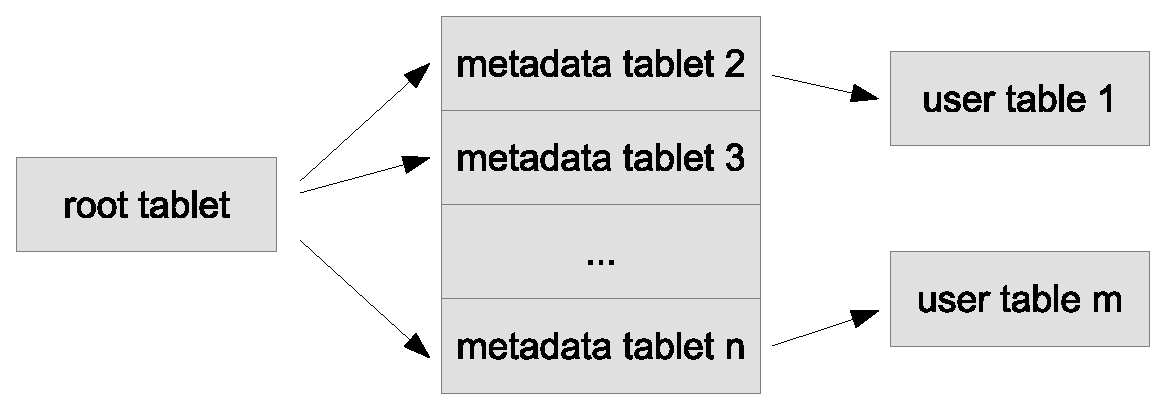
\includegraphics [width=0.7\textwidth]{images/bigtable_tablets_hierarchy}
  \caption{Bigtable tablets hierarchy}
  \label{fig:bigtable_tablets_hierarchy}
\end{figure}

\mnote{SSTable}
Bigtable stores data in special file format called SSTable.
Each SSTable consists of several blocks of a fixed size (64Kb by default). 
To locate blocks it stores their indexes, that are loaded into memory on opening the SSTable.
The blocks indexes considerably decrease the lookup time.
First the binary search is performed on in-memory index to find the needed block.
Than the appropriate block is read from disk.
The whole SSTable can be loaded into memory if necessary to perform lookup and scan operations avoiding touching disk.

A tablet can be recovered using a commit log.
This log contains all the tablet updates.
The most recent updates can be obtained from a memtable - a sorted buffer in memory.
The set of SSTables stores the older updates. 
A tablet server can read the METADATA table to detect the necessary SSTables for recovering.
Than the tablet server applies all the updates in order to restore the crashed tablet. 
  
A tablet server checks the incoming read and write operations.
The operation should be well-formed and the sender should be authorized to perform a mutation.
First the server writes a valid mutation to the commit log.
Then for write operation it inserts its content to memtable.
When the size of the memtable goes beyond the given threshold, the system frozes it.
It creates a new memtable and converts the frozen one into an SSTable. 
Read operation is performed on a merged view of the memtable and corresponding SSTables.

Periodically a merging compaction on SSTables and the memtable are used to create new SSTables out of old ones.
A regular compaction merges the memtable and a few SSTables, keeping the deletion information and deleted data.
A major compaction merges all SSTables into exactly one SSTable, cleaning deletion entries.
Bigtable performes the compaction mechanism regularly to keep the system up-to-date.

The variable number of tablets makes the system flexible and therefore easy to scale.
The implementation features provide good performance and high availability.
Bigtable is successfully used in many Google products, that proves the high quality of this storage system.

% Other BigData systems:
%Malewicz - Pregel
%Melnik - Dremel
%Akidau - MillWheel

\authorsection{Facebook architecture}{SP}

Facebook is another representative company that is strongly connected with Big Data storing and processing.
The main difference is that Facebook applications often require real-time data processing, providing a user with immediate feedback.
On the contrary, for most Google applications batch processing is sufficient to make necessary computations.

\mnote{Facebook architecture}
Figure~\ref{fig:facebook_data_flow} demonstrates the data flow in Facebook architecture.
Data originates from two sources: web servers and federated MySQL instances.
Web servers generate log data, that consists of variuos events, e.g. a user clicked a link or 'liked' a photo.
The federated MySQL contains the descripting data, such as the time of posting the link and the place where it was done.

\begin{figure}
  \centering
  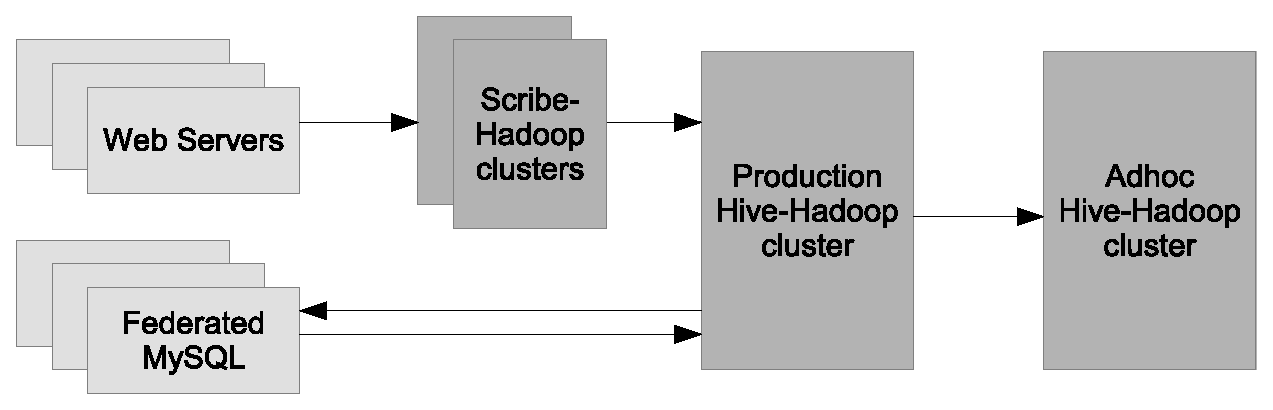
\includegraphics [width=0.9\textwidth]{images/facebook_data_flow}
  \caption{Data flow in Facebook}
  \label{fig:facebook_data_flow}
\end{figure}

Data flow goes from web servers to Scribe-Hadoop clusters.
Such cluster is actually a Hadoop cluster with a running Scribe server on the top of it.
The main function of Scribe is to aggregate the input data and write it into HDFS.
This data is transferred uncompressed [Data Warehousing and Analytics Infrastructure at Facebook] that can be a bottleneck for the whole system.
Facebook alleviates the problem by putting Scribe-Hadoop close to web servers, decreasing the network transfer load.
Periodically Scribe-Hadoop clusters send compressed data (mostly as HDFS files) to Hive-Hadoop clusters.
It is loaded to Hive and becomes available for other modules.

Scrape processes load data from federated MySQL to Hive-Hadoop cluster.
They get a dump of needed data from database, compress it and move it to the cluster.
This process should be resilient and avoid putting extra load on the databases.
The former is accomplished by using the previous days data when the database is not reachable at the moment.
To meet the latter requirement, scrape process runs on a MySQL database replica.

There are two types of Hive-Hadoop clusters - a production cluster and an adhoc one.
The purpose of the production cluster is to execute high prioriy tasks with strict deadlines.
On the contrary, the ad hoc cluster processes batch jobs with low priority and makes ad hoc analysis.
These tasks are separated, because it can be dangerous to run ad hoc user query on a production cluster.

When the data is needed for both clusters, it is replicated from the production to the adhoc cluster.
It is done in this order, because the data should be available earlier for critical jobs on the production server.
Moreover, the production server is more reliable.
During the replication process the data is transferred in a raw form accompaned by the respective metadata.

The stored data can be either transformed or queried by users.
Most of the time Hive-Hadoop clusters keep the data for future analysis.
However, in some cases the federal MySQL tier gets the data back.
This data can be uploaded on the Facebook site and participate in the further interaction with Facebook users. 

The amount of data stored on a Hive-Hadoop server is huge.
That is why Facebook compresses it using gzip.
Moreover, a special row columnar compression is used to store data in Hive.
Also Facebook uses erasure codes to provide fault tolerance and at the same time decrease the amount of data copies stored on different machines.
Erasure coding is a technique when the messages of length \textit{n} are transformed into the longer messages of length \textit{m}.
This expanded data is spread across several locations.
Later on it is possible to recover the original message using only a subset of \textit{m} symbols.

Facebook widely uses such technologies for distributed data warehousing and computation as HDFS, Hive and Scribe. 
While HDFS is an exterior module, Hive and Scribe were initially developed at Facebook and only later became open-source under the Apache Software Foundation.
HDFS is described in detail in Chapter 7 (Components), Hive and Scribe are presented in the following sections.

\mnote{Hive}
Hive is a framework designed for storing data.
Facebook uses it to query and analyze data.
Hive provides an SQL-like interface for accessing the data from Hadoop.
This makes the process of development easier comparing with a direct interaction with Hadoop via map-reduce.

Figure~\ref{fig:hive} presents the Hive structure.
Hive has a \textit{Metastore} that stores mappings between Hive and Hadoop.
The \textit{Driver} communicates with the Metastore and uses the obtained information for converting Hive query language (HiveQL) expressions into map-reduce jobs.
Hive provides various types of interfaces for interaction: web based Graphiclal User Interface (GUI), a command line, Open Database Connectivity (ODBC), Java Database Connectivity (JDBC).
The latter two communicate with the Driver using Thrift server, that represents a communication protocol for performing remote procedure calls in numerous programming languages.

\begin{figure}
  \centering
  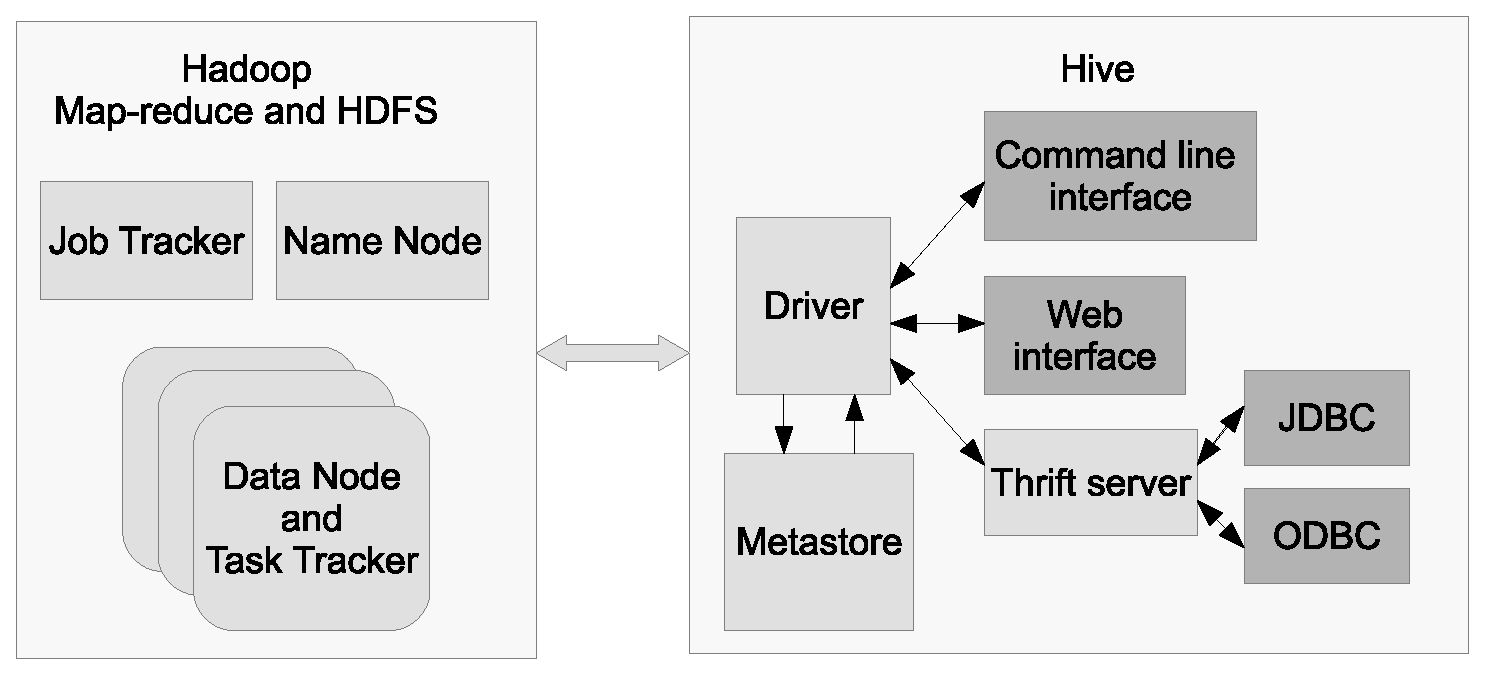
\includegraphics [width=0.9\textwidth]{images/Hive}
  \caption{Hive structure}
  \label{fig:hive}
\end{figure}

The Driver applies several types of optimization during the compilation process.
First, it uses file pruning and filtering to reduce the amount of data that should go to map-reduce jobs.
Then it uses column pruning to exclude columns that are not needed for the query.
Also the Driver uses such aggregations as 'group by' or 'join' for optimization.
Join techniques vary in the effect they have on the way of processing data.
For instance, reordering join allows to stream large tables to a reduce task avoiding helding it in memory.

Hive is a flexible framework and can be customized for the user needs.
A user can define functions, table functions or scripts written in HiveQL.
Moreover, it is possible to define custom types and data formats.

\mnote{Scribe}
Scribe is a distributed logging system designed for logging huge amounts of data. %[https://github.com/facebookarchive/scribe/wiki]
It can be spread to thousands of nodes.
At the same time it guarantees fail tolerance in the case of network or node crashes.

There are two types of servers in Scribe: general servers and central servers.
They are connected by a directed graph.%[https://www.facebook.com/note.php?note_id=32008268919]
In this graph each node knows only the next node and is not aware about the others.
This makes the communication easier, because it saves the sender from the necessity to know the network topology.

The servers interact via messages.
The data model of Scribe is simple, without timestamping, message ordering, logging levels, etc.
A message in Scribe consists of two strings: a category and a message itself.
A category reflects the message topic.
It is implied that the messages in one category have the same destination.
Categories allows to move a data store without changing a client code.
For this purpose Scribe uses the server configuration settings.
Moreover, the server can be configured to put into the file path a category name.
The message string contains the information that should be logged.

Scribe provides fault tolerance in the case of a network or machine failure as follows.
The servers send messages to the central server/servers.
Central servers, in their turn, write messages to the final destination, such as Network File System (NFS) or distributed filesystem.
When the server cannot send a message to the central server because of the network problems or the central server crash, it stores this message locally.
With random time intervals it tries to reestablish the lost connection.
To prevent the central server overload when it recovers after the failure, it can reply with the TRY LATER message.
In this case the receiver must wait several minutes before the next attempt.
The central server follows the same logic when it cannot connect to the distributed filesystem or NFS. 

However, there are some scenarios that can lead to the data loss.
For example, when the server or the central server is not available from the client side.
Or in the case of the central server crash it loses the information that was not written on disk and was kept in memory at that moment.
Or when the local disk capacity is exceeded while the central server is not available.

Scribe is based on Thrift, a software stack designed for code generation for RPC in multi-language environment.
It allows to use different languages like PHP, C++, Java or python for working with it.
The detailed discussion about Thrift is presented in Chapter 7 (Components). 
Thrift reach functionality solves many hard problems connected with logging, extending Scribe capabilities.

Scribe configuration files specify which store should be a destination for a particular directory.
There are various types of stores.
Some of them consists of other stores, like a batch store, that is build of a number of file stores.
The configuration file has a section for every store along with a global section.
Such setting as the maximum message number per second or the listening port are stored in the global section.
All the store sections contains information about a type and a category.
The number of categories is not limited as well as the number of stores for one category.
Also the store section can include specific settings that are needed for a particular store type, like maximum size of a file or its location.

\mnote{Databee}
Facebook uses Databee for managing job dependencies.
Databee is a framework written in python.
Its aim is to make the interaction process between parts of the system easier.
For example, it transmitts data from one part of the system to another, transforms data and allows to run queries on it.
Also Databee creates monitoring information, that contains such details as job latency or job completion time.
It allows to specify dependency on some data set.
Thus it is possible to run a job at the time when a needed data set becomes available.

As Facebook supports both ad hoc and periodic batch jobs, it needs a proper mechanism for sharing resources.
Periodic jobs, in contrast to ad hoc ones, have strict deadlines.
At the same time, it can happen that a long running periodic batch job blocks a short ad hoc query, holding the resources.
For the purpose of the proper sharing Facebook introduces Hadoop Fair Share Scheduler.
It divides users into pools and each of these pools are provided by the same quota of resources.
This scheduler limits the amount of concurrent jobs running in one pool.
The periodic batch jobs have their own pools.
It is guaranteed that even in the case of high load these pools are provided at least a minimum quota of resources.
Hadoop Fair Share Scheduler keeps track of the CPU and memory consumption by every node in a cluster.
The scheduler is able to kill a job that consumes memory more than allowed threshold.

\mnote{HDFS in Facebook}
[Apache Hadoop Goes Realtime at Facebook]
In matters of warehousing Facebook relies on HDFS.
This file system provides a reliable, extensible and highly available store.
However, for use cases, specific for Facebook, it has a significant disadvantage.
It is designed for batch processing, while Facebook needs a system that can handle data in real time.
Therefore a number of enhancements were introduced to make HDFS more suitable for the existent requirements.

HDFS has a node called NameNode, that serves as a master node for the cluster.
To prevent NameNode being a single point of failure, HDFS uses a BackupNode.
In the case of failure the schema works as follows.
First, a NameNode reads a metadata file, recreating a file system image.
Second, a NameNode waits for the replies from DataNodes, that should report about their location.
The presence of the BackupNode helps to avoid the first step.
The BackupNode stores the copy of the file system image.
Nevertheless, the second step is still necessary and takes considerable time to complete.

To make the cold-start process fast, Facebook introduces an AvatarNode.
There are two AvatarNodes in a cluster.
One of them is an Active AvatarNode, that represents a wrapper around a NameNode.
The second one is a hot-standby copy of the former.

Figure~\ref{fig:facebook_avatarnode}  illustrates how two AvatarNodes interact with each other.
The Active AvatarNode stores a filesystem image and a transaction log in a Network file system (NFS).
Simultaneously the Standby node reads this information and applies all the transactions.
DataNodes send the location information to both Active and Standby node.
Thus the Standby node can replace the Active one at any moment.
Facebook also modified the transactions form, enriching it with id, data length and a checksum.
This helps to avoid reading a partial transaction by the Standby AvatarNode.

\begin{figure}
  \centering
  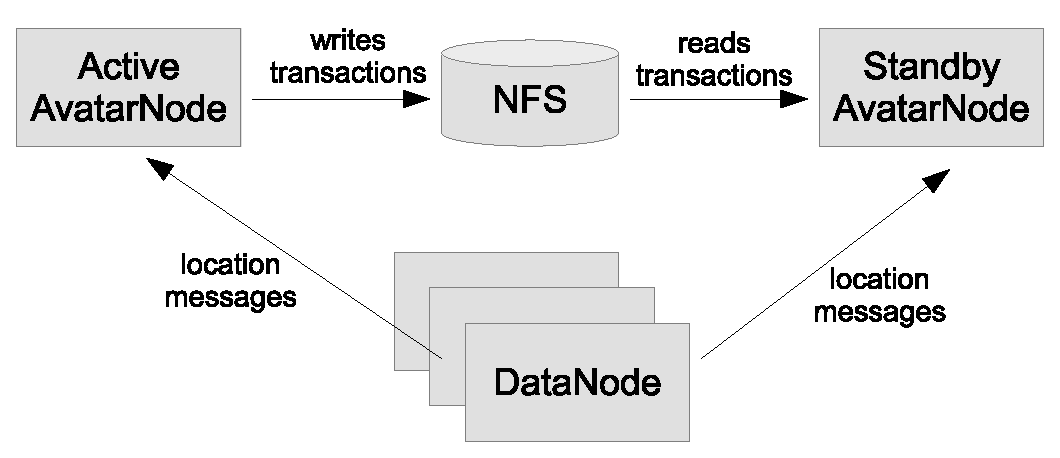
\includegraphics [width=0.7\textwidth]{images/facebook_avatarnode}
  \caption{AvatarNodes interaction}
  \label{fig:facebook_avatarnode}
\end{figure}

Facebook has improved an RPC mechanism.
As the company controls the huge number of machines, it should be able to cope with a situation when different clusters have different Hadoop version installed.
Therefore the implementation of RPC was changed.
It became possible to detect the Hadoop version automatically and use the appropriate protocol for communication.
Also Facebook added a possibility to specify an RPC timeout.
Originally, Hadoop was designed in such a way that the client is waiting for the reply from an RPC server infinitely.
However this is inadmissible for real-time applications.

HDFS was extended by \textit{recoverLease} API, that significantly decreases the lease revokation time.
Before this enhancement HDFS used a soft lease mechanism.
In this case, when the clien cannot read the file, it continues read tries until success or until the soft lease expires (that was one minute by default).
Due to the \textit{recoverLease} it becomes possible to revoke a lease immediately.
A \textit{recoverLease} request is received by the NameNode.
At that moment it becomes a holder of the file and starts to recover the lease.
When it is done, the NameNode replies with 'recovery complete' message.
Then the client can start reading from the file.

\mnote{HBase}
Facebook uses HBase as a database. 
HBase is a distributed database that is built on a basis of BigTable and runs on top of HDFS.%[http://hbase.apache.org/book/architecture.html]
HBase can be called as one of the implementations of BigTable, therefore it has an identical structure.

Facebook optimizes the database for its own needs.
For example, to improve write performance, the following steps are applied.
First, data is stored into a commit log.
Then it goes to Memstore, an in-memory cache.
Memstore gathers data until it reaches a limit and then write it as an HFile to HDFS.
HFile is a file format for HBase, that contains a sorted set of key-value pairs.
With every flush operation a new HFile is created.
Thus these files should be merged periodically for better read performance.
This process is called files compaction.

\mnote{Haystack}
Haystack is another technology used by Facebook to solve problems of large-scale data.
It is an object storage system designed for working with billions of files.%[Finding a needle in Haystack: Facebook�s photo storage]
Facebook uses it for photo warehousing.

Photo storing differs from other storage system applications.
The storage system writes a photo only once and never modifies.
Also photos are read quite often.
Photos do not need most of the metadata information usually stored by a file system for each file.
Moreover, Facebook requires a fast way to find and read a photo.

Haystack is specifically designed to meet all the Facebook requirements.
Figure~\ref{fig:haystack_architecture} shows the Haystack architecture.
The main three parts of Haystack are Haystack Directory, Haystack Store and Haystack Cache.
The Store contains photos and associated metadata.
The Store is devided into logical volumes, each of them combines several physical volumes.
The Directory is responsible for mapping between logical and physical volumes.
The Cache is a content delivery network (CDN), that provides access for most frequently asked photos.

\begin{figure}
  \centering
  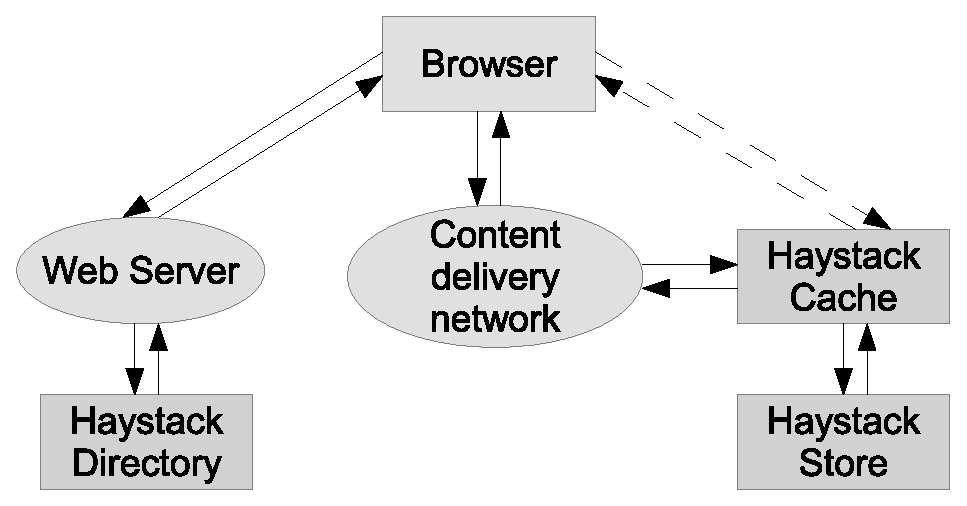
\includegraphics [width=0.5\textwidth]{images/haystack_architecture}
  \caption{Haystack architecture}
  \label{fig:haystack_architecture}
\end{figure}

The typical scenario of a user-Haystack interaction can be described as follows.

1. The user visits a page that contains some photos.

2. The web server receives a request from the browser and asks the Directory for the photo URL.
The URL has the following structure: http://[CDN]/[Cache]/[Machine id]/[Logical volume, Photo id] %[Finding a needle in Haystack: Facebook�s photo storage]

3. The browser communicates with the CDN specified in the URL. 
In some scenarios the browser communicates directly with the Cache, passing over the CDN.

4. The CDN searches for the photo locally, using the Logical volume and Photo id information.

5. If the photo is not found, the CDN transfers the request to the Cache.

6. The Cache performs the same actions and if the photo is still not found, it asks the Store machine.

When the user uploads a photo:

1. The web server askes the Directory for the logical volume where the photo can be written.

2. Then the server assignes an id to this photo.

3. Finally it saves the photo on every physical volume assiciated with the given logical module. 
 
\mnote{Haystack Directory}
The Directory has four main applications in Haystack.
First, as it was mentioned, the Directory manages a mapping between logical and physical volumes.
Second, it performs the load balancing.
The Directory controls the write and read load among logical and physical volumes correspondingly.
Third, it determines read-only logical volumes.
A logical volume becomes read-only, for example, when it does not have free memory for storing new photos.
Forth, the Directory specifies which component (CDN or Cache) should be used by the browser.    

\mnote{Haystack Cache}
The Cache is a distributed hash table.
Haystack uses a photo id as a key to obtain the needed photo.
The Cache stores the photo only when it receives a request directly from a browser, not from the CDN.
Also it is necessary that the photo is located on a write-enabled machine.

\mnote{Haystack Store}
Every Store machine contains several physical volumes.
One such volume can be considered as a very large file, containing millions of photos.
This is done to decrease the amount of metadata stored for each file.
To obtain the photo, the Store needs a logical volume id and the file offset.
The Store keeps in memory the mapping between the photo id and its offset, size and other metadata information.
This allows to make the process of photo retrieving fast.

A physical volume consists of a sequence of needles, where one needle is associated with one photo.
Each needle contains: a Header with information for recovery, a Cookie to prevent brute force lookups, a Key and an Alternative key, Flags showing deletion status, a Size, the Data itself, a Footer also used for recovery, a Checksum and a Padding.
The Key is represented by the photo id and the alterative key by its type.
The type in this case denotes the size - each photo on upload is scaled to four different sizes.
The cookie is a number randomly assigned by the Directory.
It is added to the photo URL and prevents attacks for guessing the URL.

There are three actions that the Store can perform with a photo.
First, the photo can be written.
A Cache machine sends a request to Store machines, containing a key, an alternative key, a logical volume id, a cookie and the data to be stored.
Every store machine saves the data and updates mapping that are stored in memory.
The Store supports only append operation, so the data once written cannot be modified.
Thus when a new version of a photo should be stored, the Store adds an updated niddle that has the same key and alternative key.
Different versions are distinguished by different offsets in a file.

Second, the Store allows to read photos.
A Cache machine sends the same data as with writing, except the data to be stored.
The store searches for the necessary metadata in memory.
The Store finds the necessary file and seeks for the specified offset in it.
It reads the appropriate needle.
Finally some verifications like cookie check or data integrity are performed. 

Third, a photo can be deleted.
When the photo is deleted, the Store sets two flags: one for in-memory mapping and one for the volume file.
If the Store receives a request for a deleted photo, and the in-memory flag is set to 'deleted', the Store returns an error.
Deleted needles still occupy the space on disk, so it is released using the file compaction.

Haystack uses an \textit{index file} for optimizing the time of Store machines reboot.
The problem is that every machine has to restore its in-memory mappings.
Instead of inspecting all its physical volumes on reboot, a Store machine reads the index file.
The index file has the similar structure to physical volume files.
It contains a set of records, where one record corresponds to one needle.
It is important that the ordering of records should be the same as the ordering of needles.
The index file has the following fields: Key and Alternate key, Flags, Offset and Size.

When a photo is written into the Store, the index file is updated asynchronously.
When a user deletes a photo, the index file is not changed at all.
This is done to improve the performance.
However, it brings some problems: (1) it is possible to have a needle without a related index record, (2) index file has no information about deleted photos.
The needle that has no record in index file is called an \textit{orphan}.
The Store machine gets rid of orphans during the reboot process: for each orphan needle it creates a record in the index file.
To solve the second problem, the Store checks the deleted flag on receiving a read request.

Haystack uses a background task called \textit{pitchfork} to recover from failures.
This task is responsible for checking the state of all the Store machines peroidically.
It should check the connection, volume files availability and the ability to read data.
If the tests are failed, all the logical volumes of this machine are marked as read-only.
Then such machines are manually examined to find the reason of failure.    

 







% 1. Flow of data (Data Warehousing and Analytics Infrastructure at Facebook)
% 2. HDFS enhancement + HBase + Hive + Scribe (Data Warehousing and Analytics Infrastructure at Facebook) + (Apache Hadoop Goes Realtime at Facebook)
% 3. Haystack (https://www.facebook.com/note.php?note_id=76191543919) + (Finding a needle in Haystack: Facebook�s photo storage)
% 4. jemalloc (https://www.facebook.com/notes/facebook-engineering/scalable-memory-allocation-using-jemalloc/480222803919)